\newpage
\section{Auswertung}
    Das gemessene Autokorrelationssignal des unmodulierten Lasers ist zusammen mit dem vermessenen Spektrum in Abbildung \ref{fig:normal} zu sehen. Das Spektrum weist ein Hauptmaximum bei $\sim \SI{1550}{\nano\metre}$ auf, wie vom Lasersystem zu erwarten, und weitere kleinere Peaks bei Wellenlängen von $\pm \SI{50}{\nano\metre}$ auf.
    \begin{figure}
        \centering
        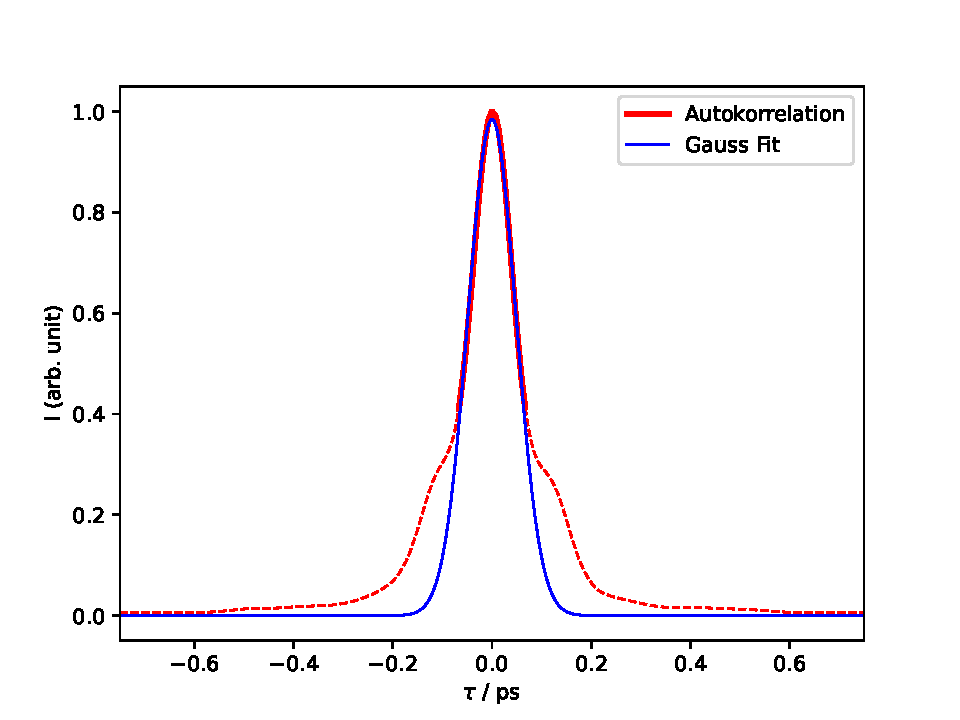
\includegraphics[width = 0.45\textwidth]{pictures/Puls_normal.pdf}
        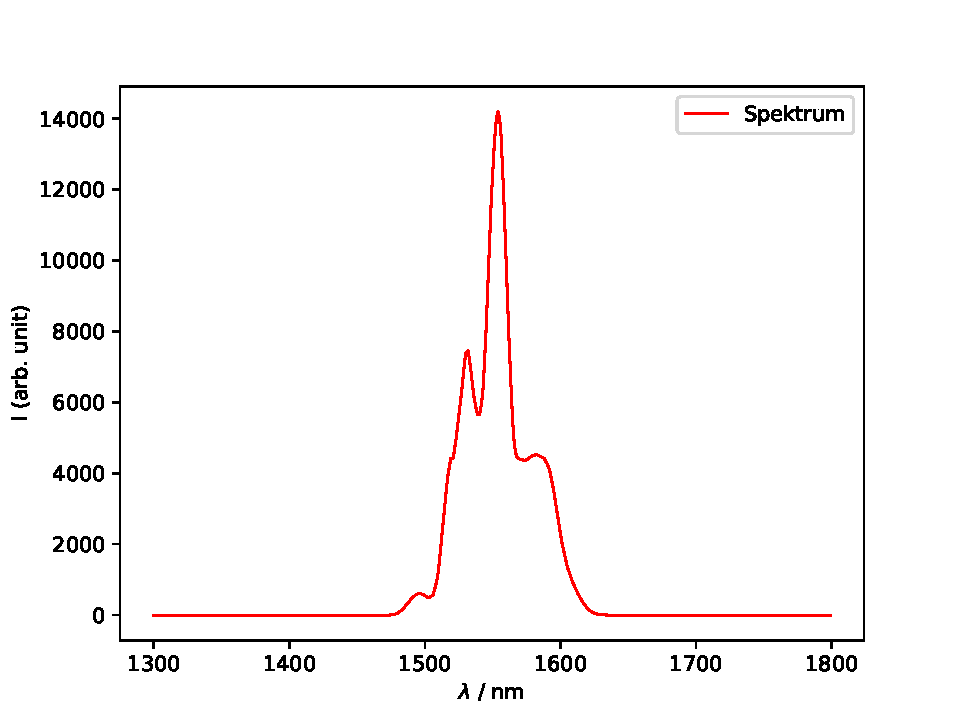
\includegraphics[width = 0.45\textwidth]{pictures/Spektrum_normal.pdf}
        \caption{\textit{Links:} Autokorrelationsspur des Lasers (rot). Die durchgezogene Linie zeigt den Bereich an, an dem der Gauß-Fit (blau) durchgeführt wurde. \textit{Rechts:} Spektrum des Lasers.}
        \label{fig:normal}    
    \end{figure}
    Obwohl der Puls als gaußförmig angenommen wird, weißt die Autokorrelationsspur neben einem Peak in der Mitte zwei Schultern auf. Diese werden Satelliten zugewiesen und werden in der Folgenden Brechnung ausgeschlossen. An dem gaußförmig Bereich der Spur wird, wie in Formel \ref{eqn:IntGauss} beschrieben, ein Gauß-Fit der Form
    \begin{equation}
        I(x) = A \cdot \exp\left(-4\ln(2)\left(\frac{\tau}{\Delta \tau_{AK}}\right)^2\right)
    \end{equation}
    durchgeführt. Dieser ist ebenfalls in Abbildung \ref{fig:normal} dargestellt und liefert nach Formel \ref{eqn:tautau} eine Pulsdauer von
    \begin{equation}
        \Delta \tau^{\text{Laser}} = (80.41\pm 0.92)\,\text{fs}
    \end{equation}
    Die Diskussion der Ergebnisse und der Vergleich mit den erwarteten Werten erfolgt in Kapitel \ref{sec:Dis}.
    \subsection{Pulsdauer mit Bandpassfilter}
        Auch hier wird das Spektrum und die Autokorrelationsspur betrachtet. In Abbildung \ref{fig:30} sind diese für den $\SI{30}{\nano\metre}$-Filter zu sehen.
        \begin{figure}
            \centering
            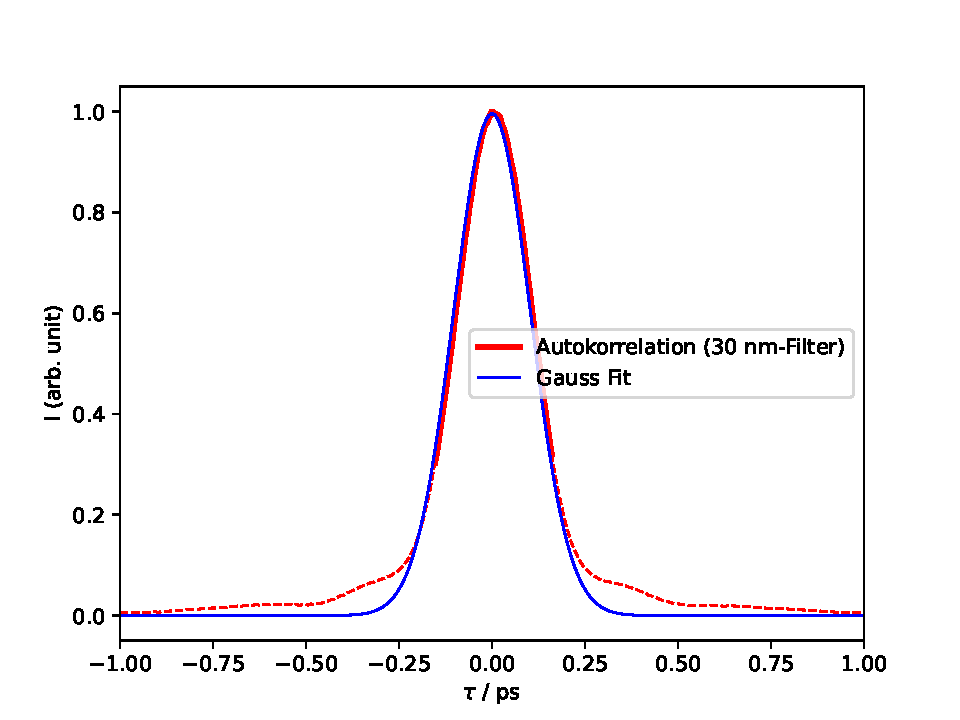
\includegraphics[width = 0.45\textwidth]{pictures/Puls_30.pdf}
            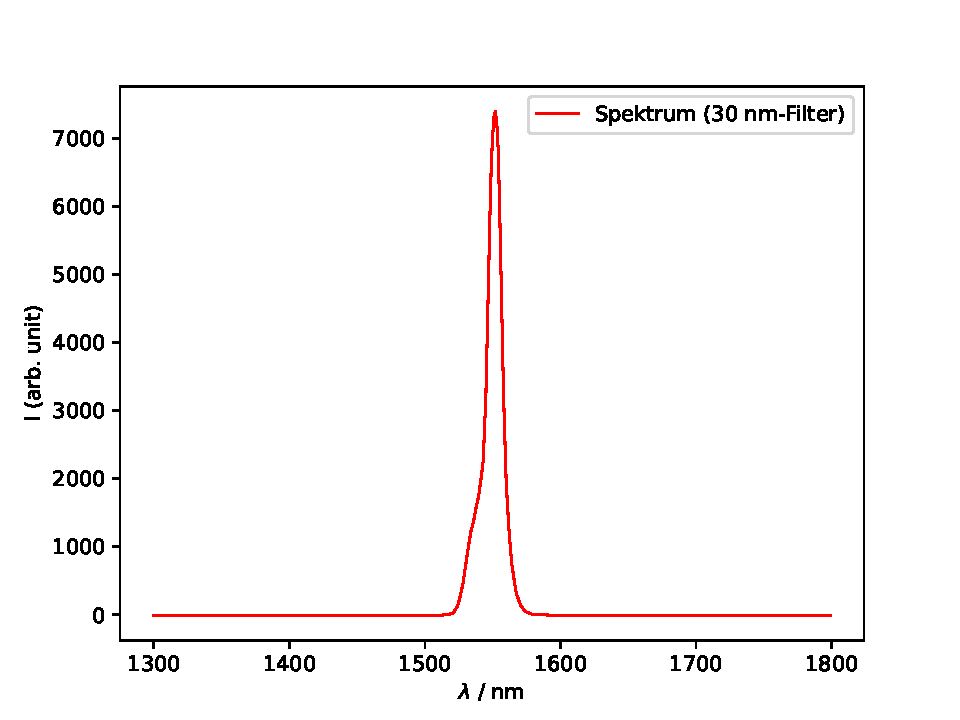
\includegraphics[width = 0.45\textwidth]{pictures/Spektrum_30.pdf}
            \caption{\textit{Links:} Autokorrelationsspur des Lasers mit $\SI{30}{\nano\metre}$-Bandpassfilter (rot) und Gauß-Fit (blau). \textit{Rechts:} Spektrum des Passieren des Filters.}
            \label{fig:30}    
        \end{figure}
        Im Spektrum gibt es, wie zu erwarten, nur noch Beiträge unmittelbar um die zentrale Wellenlänge, da nur die Wellenlängen in einem Bereich von $\pm \SI{30}{\nano\metre}$ durch den Filter transmittiert werden. Auch hier wird wieder ein Gauß-Fit an den 'satelliten-freien' Teil des Autokorrelationssignals gelegt (siehe \ref{fig:30}) und aus dem Fit-Parameter und mit Hilfe von Formel \ref{eqn:tautau} die Pulslänge bestimmt. Diese ergibt sich für den $\SI{30}{\nano\metre}$-Filter als
        \begin{equation}
            \Delta \tau^{\text{30nm}} = (171.33\pm 1.76)\,\text{fs} \, .
        \end{equation}

        Für den $\SI{12}{\nano\metre}$-Bandpassfilter ergibt sich im Spektrum ein noch schmalerer Bereich mit einem Beitrag. Für die Pulsdauer in diesem Fall ergibt sich
        \begin{equation}
            \Delta \tau^{\text{12nm}} = (287.27\pm 1.51)\,\text{fs} \, .
        \end{equation}
        nach dem selben Analyseverfahren für zuvor. Der Gauß-Fit ist zusammen mit dem Spektrum in Abbildung \ref{fig:12} gezeigt.
        \begin{figure}
            \centering
            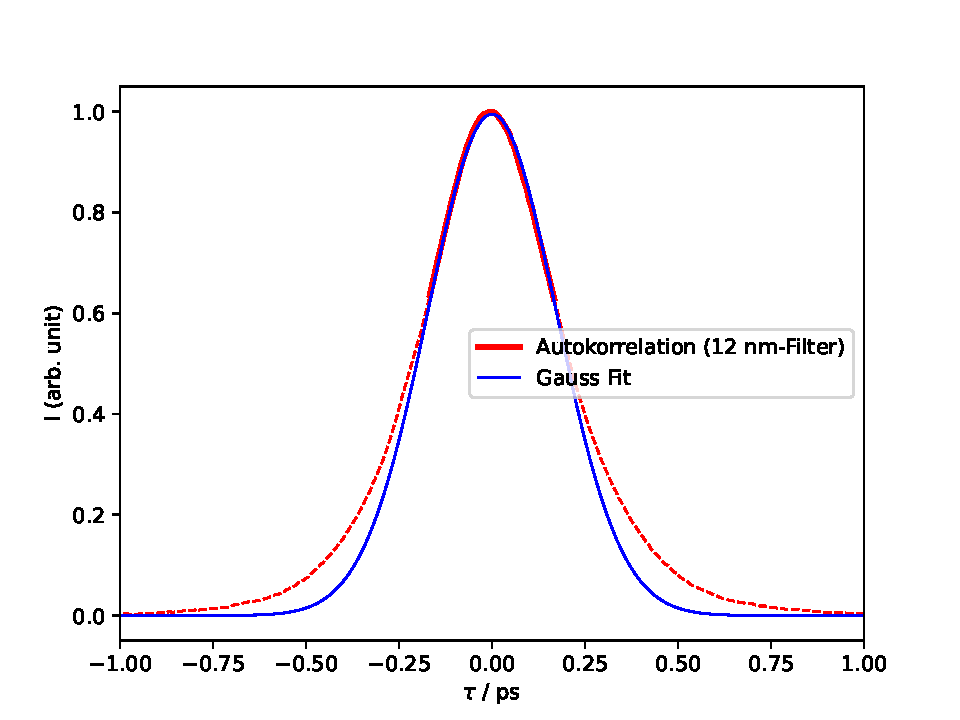
\includegraphics[width = 0.45\textwidth]{pictures/Puls_12.pdf}
            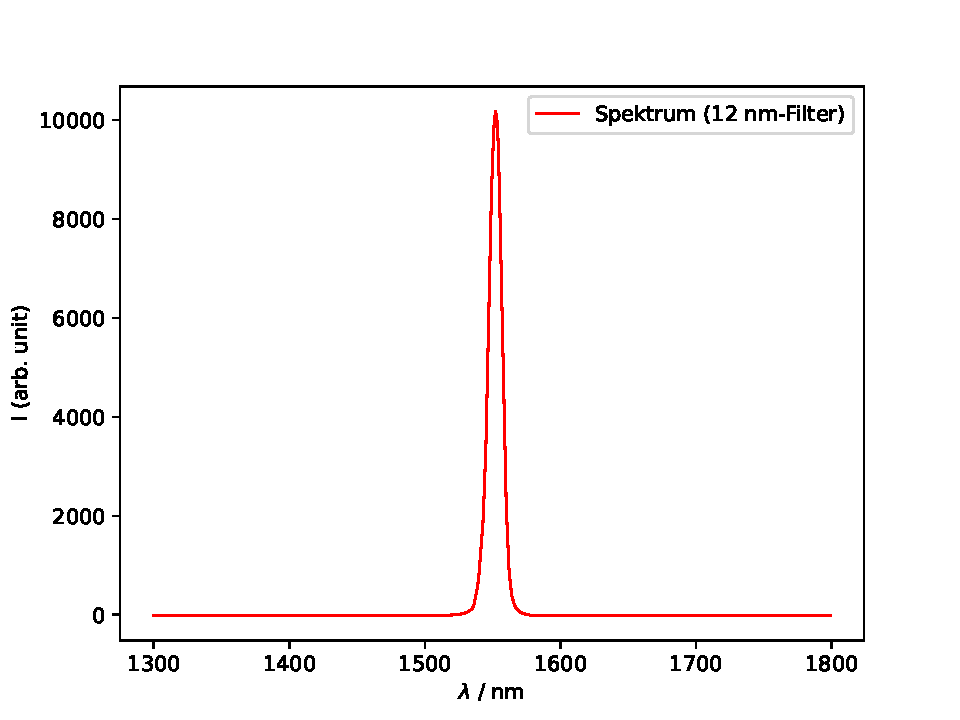
\includegraphics[width = 0.45\textwidth]{pictures/Spektrum_12.pdf}
            \caption{\textit{Links:} Autokorrelationsspur des Lasers mit $\SI{12}{\nano\metre}$-Bandpassfilter (rot) und Gauß-Fit (blau). \textit{Rechts:} Spektrum des Passieren des Filters.}
            \label{fig:12}    
        \end{figure}
        Auch hier werden die Ergebnisse in Kapitel \ref{sec:Dis} besprochen.
    \subsection{Pulsdauer mit dispersiven Medien}
        Das gemessene Autokorrelationssignal für den Laser nach Durchlaufen des $\SI{12}{\milli\metre}$ langen Silizium-Blocks ist in Abbildung \ref{fig:Si} aufgetragen.
        \begin{figure}
            \centering
            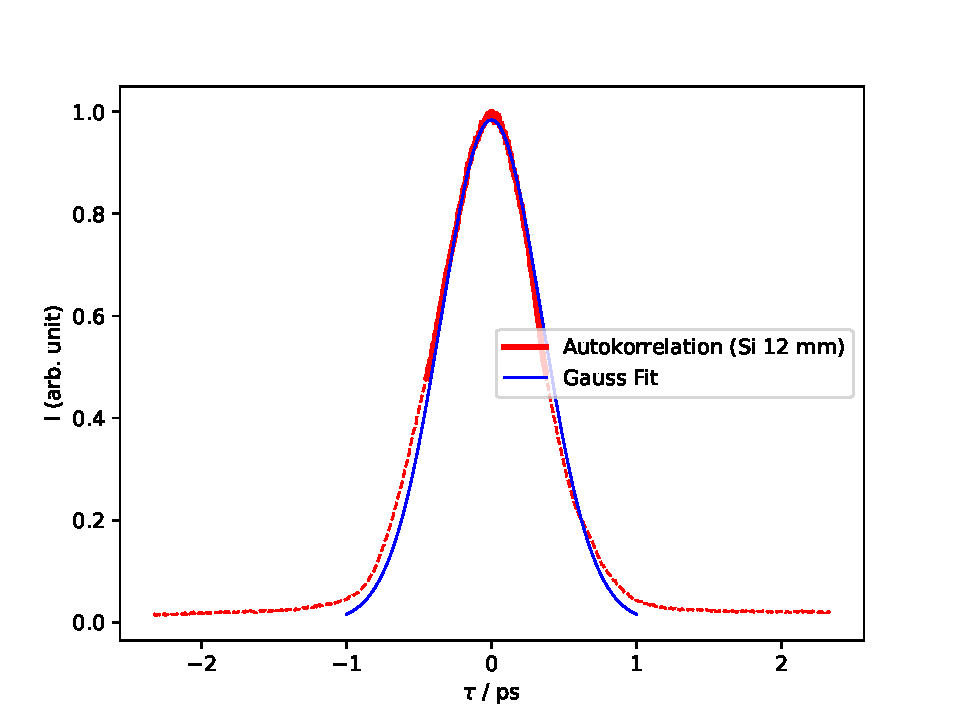
\includegraphics[width = 0.8\textwidth]{pictures/Puls_Si.pdf}
            \caption{Autokorrelationsspur des Lasers nach Propagation durch Silizium (rot) und Gauß-Fit zur Bestimmung der Pulsdauer (blau).}
            \label{fig:Si}    
        \end{figure}        
        Die gefittete Gauß-Funktion ist ebenfalls dargestellt und führt zu einer Pulsdauer von
        \begin{equation}
            \Delta \tau^{Si} = (578.45\pm 4.35)\,\text{fs} \, .
        \end{equation}
        
        Die Pulsbreite wird als nächstes für die 5 unterschiedlichen Glassblöcke bestimmt. Der Übersichtlichkeit halber sind in Abbildung \ref{fig:Glass} lediglich die Gauß-Fits für die verschiedenen Dicken aufgetragen.
        \begin{figure}
            \centering
            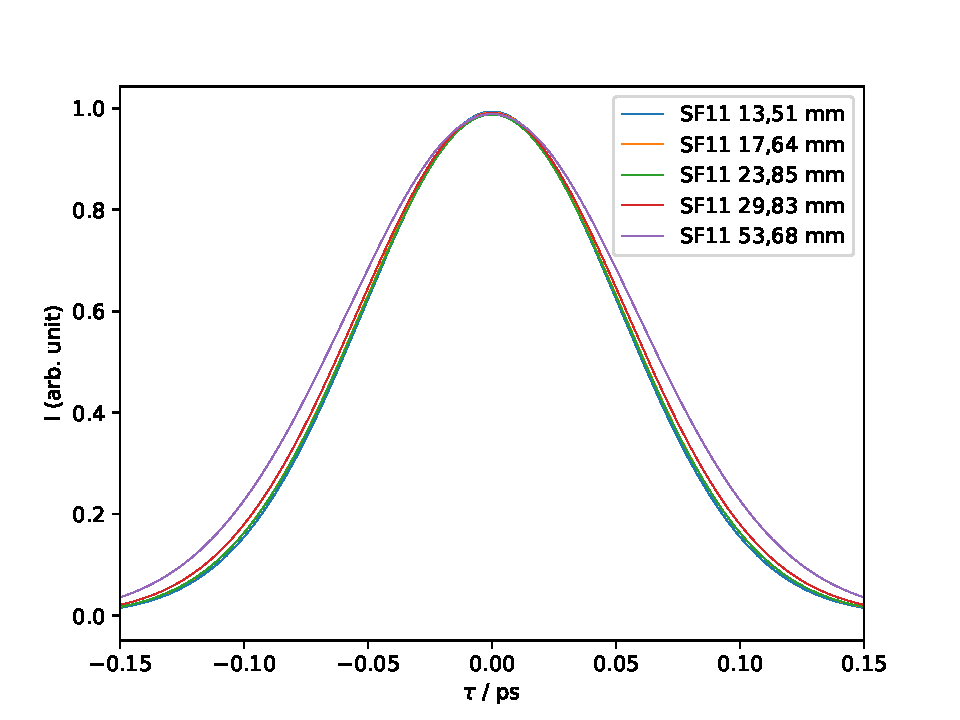
\includegraphics[width = 0.8\textwidth]{pictures/Puls_Glass.pdf}
            \caption{Gefittete Gauß-Funktionen zur Bestimmung der Pulsdauer für die unterschiedlichen Glassblock-Dicken.}
            \label{fig:Glass}    
        \end{figure}        
        Diese werden wie zuvor beschrieben aus den gemessenen Autokorrelationsspuren ermittelt. Es ist eine leichte Verbreiterung des Gauß-Fits mit zunehmender Dicke der Glassblöcke zu erkennen. Die daraus bestimmten Pulsdauern sind in Tabelle \ref{tab:Dauer} aufgelistet.
        \begin{center}
            \captionof{table}{Pulsdauern des Lasers nach Propagation durch die unterschiedlichen Glassblock-Dicken.}
            \label{tab:Dauer}
            \begin{tabular}{c c}
                \toprule
                Dicke / mm & Pulsdauer $\Delta\tau$ / fs \\
                \midrule
                $13.51$ & $(86.34 \pm 0.75)$ \\
                $17.64$ & $(87.63 \pm 1.14)$ \\
                $23.85$ & $(87.71 \pm 1.25)$ \\
                $29.83$ & $(90.10 \pm 0.48)$ \\
                $53.68$ & $(97.06 \pm 0.86)$ \\
                \bottomrule
            \end{tabular}
        \end{center}

